\begin{table}[]
\begin{tabular}{llrr}
\textbf{Domain} & \textbf{Model} & \textbf{Params} & \textbf{TBS} \\ \hline
CV  & ResNet18~\cite{he2015deep} & 11.7M  & 8192,  16384, 32768 \\              
    & ResNet50~\cite{he2015deep}  & 25.6M  &  \\              
    & ResNet152~\cite{he2015deep} & 60.2M  &  \\              
    & WideResNet101\_2~\cite{zagoruyko2016wide} & 126.9M &  \\              
    & ConvNextLarge~\cite{liu2022convnet} & 197.8M &  \\ \hline
NLP & RoBERTaBase~\cite{liu2019roberta}  & 124.7M & 8192,  16384, 32768 \\
    & RoBERTaLarge~\cite{liu2019roberta} & 355.4M &  \\
    & RoBERTaXLM~\cite{conneau2020unsupervised} & 560.1M &  \\
\end{tabular}
\caption{Model suitability parametrization.}
\label{tab:experimental-setup-for-model-suitability}
\vspace*{-10mm}
\end{table}
Selecting suitable models with a big enough parallel workload is essential to ensure successful distributed spot training.
To cover a wide range of established models, we drew from MLCommons' comprehensive DL training benchmark~\cite{mattson2020mlperf}.
We used models from the CV and NLP domains and gradually increased their size and TBS to increase the parallel compute amount (\Cref{tab:experimental-setup-for-model-suitability}).
As discussed in ~\Cref{sec:distributed-dl}, the TBS may be exclusively responsible for the success of distributed training and was chosen to cover both medium and large batches (8K, 16K and 32K).
These minibatch sizes start to become more common due to the LAMB optimizer~\cite{you2019large}, which works well enough for both smaller (512) and huge batches (64K) and should be representative of state-of-the-art workloads.
All experiments were run with FP16 precision, as the target T4 GPUs have a considerable improvement in FLOPs compared to FP32 (8:1).

For \textbf{CV}, we take five models from the extended ResNet family, starting with the smallest one, ResNet18 (RN18), ResNet50 (RN50), ResNet152 (RN152), WideResNet101\_2 (WRN101) and end with ConvNextLarge (CONV), which has almost 20 times more parameters.
For the dataset, we use Imagenet1K~\cite{deng2009imagenet} and train the classification task, which tries to assign one of 1000 classes to each image.

For \textbf{NLP}, we selected three models from the BERT family:\\RoBERTaBase (RBase), RoBERTaLarge (RLrg), and RoBERTaXLM (RXLM).
We maintained the same configuration as the original models and trained them on masked language modeling (MLM), a common pre-training task.
The text dataset was a Wikipedia dump from March 2022~\cite{wikidump}.

When we run our experiments in a multi-cloud environment on spot instances, we cannot plug in proprietary cloud storage or wait for the dataset to download, as the instances can be terminated anytime.
To simulate a real-world deployment with a non-public dataset, we chose an independent S3 storage provider, Backblaze (B2)\footnote{https://backblaze.com/}.
Backblaze has replicated data centers that can better serve requests from anywhere worldwide, guaranteeing a reasonable ingress rate from every continent.
Additionally, the cost is very manageable at 0.01\$/GB rate for egress and 0.005\$/GB/month for storage.
A detailed analysis of the costs incurred for the experiments can be found in ~\Cref{sec:multicloud-performance}.
We access the datasets on-demand via shards in the \texttt{tar} format with the WebDataset library~\cite{aizman2019webdataset}.
We chose WebDataset due to its features like automatic local caching, streaming decompression, streaming preprocessing, and having an easy to work with archive format that allows representing the data in its original format.
Finally, for the Hivemind parameterization, we enabled delayed parameter averaging (DPU)~\cite{ren2021zerooffload} to enable simultaneous gradient communication and computation at the expense of a round of staleness. We selected FP16 compression for peer-to-peer communication.

\textbf{Experimental design.} First, we must verify that our models are suitable for cloud training.
For this purpose, we evaluate them on the powerful Ampere GPUs first - if they scale there without facing a communication bottleneck, they should also scale on the slower T4, which is common at GC, AWS, and Azure clouds.
We use the cloud provider LambdaLabs~\cite{lambdaweb} for these experiments, which gives us on-demand A10 GPUs for just 0.60\$/hour, but currently offer their services only in the US West region.
The nodes feature an Intel Xeon Platinum 8358 running at 2.60 GHz, 30 cores, and 200 GB RAM.
All experiments are performed on the 515.65.01 driver, CUDA 11.7, and PyTorch 1.13.1.
We profiled a network bandwidth of 3.3 Gbits and a latency of 0.3 ms between the Lambda VMs. 
   
To establish a fair baseline, we train all models from ~\Cref{tab:experimental-setup-for-model-suitability} on a single GPU that achieves large minibatch sizes through gradient accumulation.
Each peer logs system metrics every second and evaluates the training performance whenever a batch is processed.
Finally, all multi-GPU experiments are monitored with a training monitor that scrapes the DHT every second to log the peer state and training progress synchronously.

\textbf{(1) Hivemind penalty.} Using Hivemind as middleware to share gradients and keep a fully decentralized architecture running harms performance compared to single-node training. 
We can compare the effects of Hivemind training by looking at three metrics: \textit{baseline}, the single GPU throughput, \textit{hivemind local}, normalized GPU throughput without the averaging step, and \textit{hivemind global}, the actual normalized GPU throughput.
When comparing the baseline and local speed in ~\Cref{fig:hivemind-penalty-analysis} for a setup with two GPUs, running Hivemind reaches at best 78\% (ResNet152) and at worst 48\% (ConvNextLarge) of the baseline performance.
Unsurprisingly, the larger the model size, the worse the penalty gets due to the increased size of the accumulated gradients (GAC) over each step.
However, the baseline also applies gradient accumulation to reach the target minibatch size without the performance drop.
After isolating the respective function calls, there seems to be a slight inefficiency in how GAC is implemented in Hivemind versus the native PyTorch call.
We are working with the maintainers to fix this issue\footnote{https://github.com/learning-at-home/hivemind/issues/566}.
On the other hand, the disadvantage of synchronization is minimal under the perfect conditions of a good interconnect.
The global speed in ~\Cref{fig:cv-2xa10-local-sps,fig:nlp-2xa10-local-sps} only degrades at best to 97\% (ConvNextLarge) to at worst to 87\% (RoBERTaBase) compared to the local throughput, meaning that the communication under these conditions only accounts for a fraction of the total training time.
This degradation is inversely correlated to the model size due to larger models training quadratically longer per parameter, but the communication only increases linearly~\cite{ryabinin2023swarm}.
While an implementation issue currently affects performance, and the worst total performance drop is at 47\% (ConvNextLarge baseline vs. global), scaling is still possible with a ratio of roughly 2:1 of GPUs to throughput.
We further refine this ratio in the following section by comparing which models are most suitable to be trained in a distributed environment.
 
\begin{figure} 
    \begin{subfigure}[c]{0.238\textwidth} 
        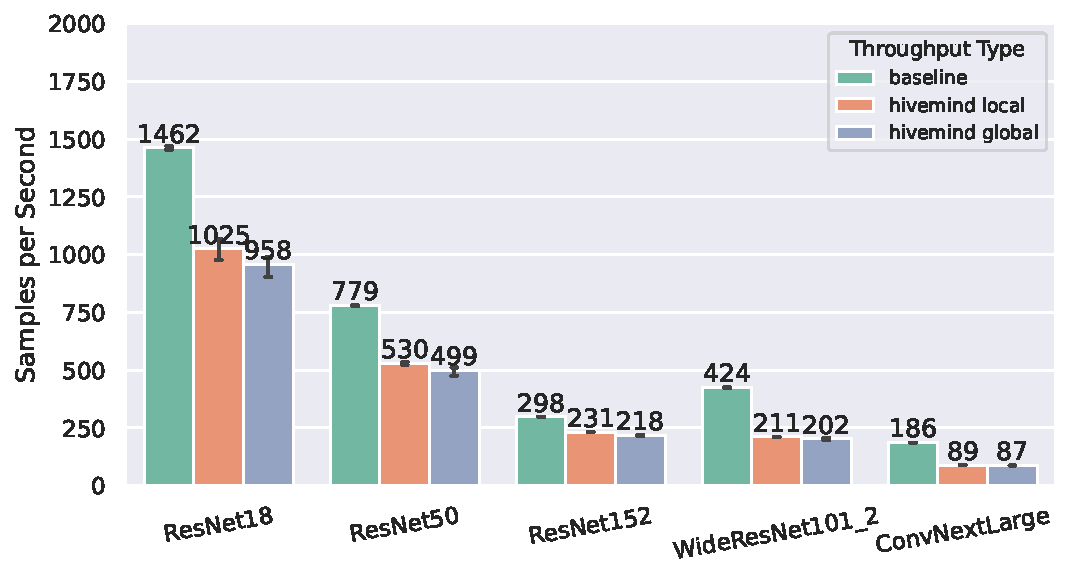
\includegraphics[width=\textwidth]{figures/misc/cv_2xa10_32768_hivemind_local_sps}
        \vspace{-20pt}  
        \caption{CV}
        \label{fig:cv-2xa10-local-sps}
    \end{subfigure} 
    \begin{subfigure}[c]{0.23\textwidth}
        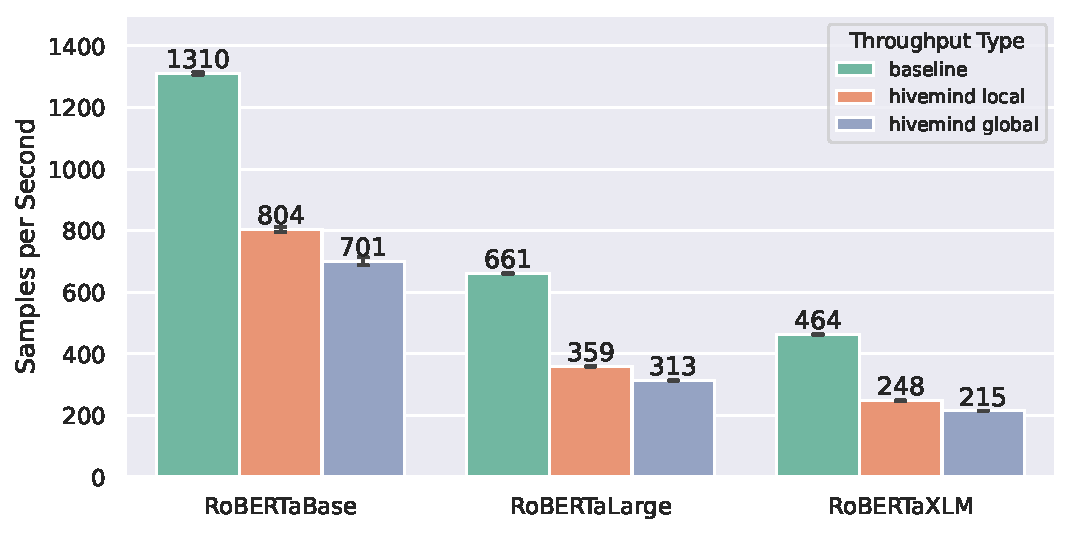
\includegraphics[width=\textwidth]{figures/misc/nlp_2xa10_32768_hivemind_local_sps}
        \vspace{-15pt}
        \caption{NLP}
        \label{fig:nlp-2xa10-local-sps}   
    \end{subfigure}
    \vspace{-13pt}
    \caption{Hivemind penalty on normalized throughputs.}
    \label{fig:hivemind-penalty-analysis}
    \vspace*{-5mm}
\end{figure}

\textbf{(2) Less suitable models for distributed spot training.} While training billion-parameter NLP models scale well due to the "square-cube" law, the minimum model size is not yet fully defined~\cite{ryabinin2023swarm}. 
The reason is that many factors play a role in whether a model is suited for geo-distributed training.
On the one hand, a small model results in small gradients exchanged between peers, so the averaging step is fast.
On the other hand, a small model will also reach the TBS faster than larger models, which may lead to a low speedup if the calculation time is disproportionally lower than the communication time.
We found the granularity metric~\cite{10.5555/541880}, typically used in high-performance computing, practical to attach a comparable value to each setup to quantify the ratio of the calculation and communication time (\Cref{eq:granularity-formula}).
The higher the granularity, the more parallelizable the task, as more calculation can be distributed between peers, ensuring a good speedup.
It is important to note that this metric depends on the model and the hardware being used. 
The communication time is affected by the parameter count, and the calculation time is affected by the layer type of the parameters (including feedforward, convolution, and transformer).
Therefore, the calculation time can decrease with improved hardware, which we evaluate in ~\Cref{sec:hybrid-cloud-performance}.
\vspace*{-1mm}
\begin{equation}
    G = \frac{T_{\text{calc}}}{T_{\text{comm}}}
    \label{eq:granularity-formula}
\end{equation}
Another parameter that affects the calculation time is the TBS that all peers work to accumulate.
There is a practical limit to the TBS where a model is still trainable, which is currently at 64K samples with the LAMB optimizer~\cite{you2019large}.
This limits the possibility of improving the speedup of small models by increasing the batch size, meaning that at some point, the speed will be limited by the communication time (\Cref{eq:time-formula}).
\vspace*{-4mm}
\begin{equation}
    \lim \limits_{T_{\text{calc}} \to 0} \frac{\text{samples}}{T_\text{comm} + T_\text{calc}} = \frac{\text{samples}}{T_\text{comm}}
    \label{eq:time-formula}
\end{equation}

\begin{figure}
    \begin{subfigure}[c]{0.23\textwidth}
        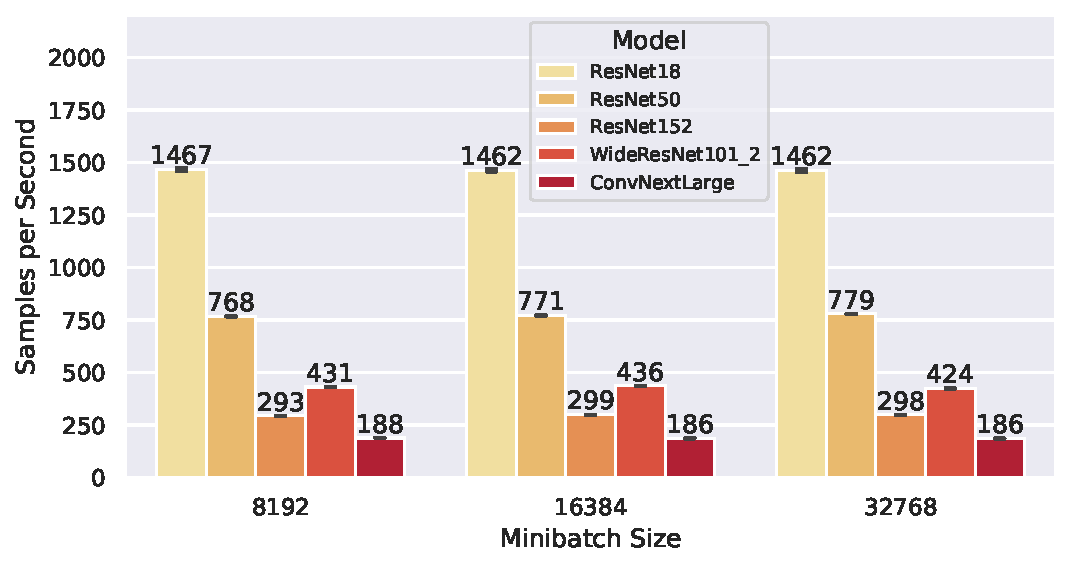
\includegraphics[width=\textwidth]{figures/misc/cv_1xa10_all-tbs_baseline}
        \vspace{-18pt}
        \caption{CV 1xA10}
        \label{fig:cv-1xa10-baseline}
    \end{subfigure}
    \begin{subfigure}[c]{0.23\textwidth}
        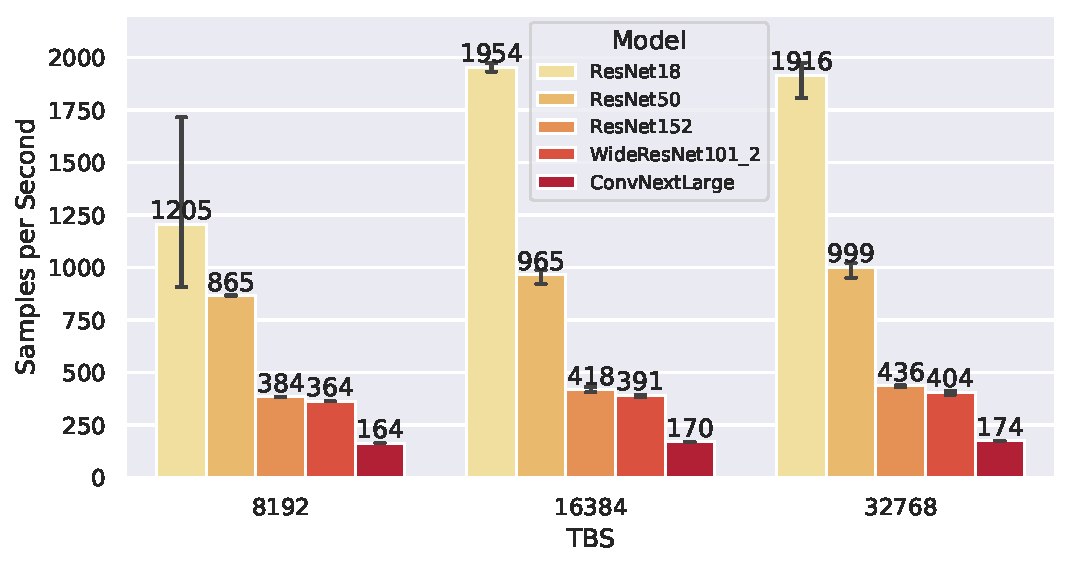
\includegraphics[width=\textwidth]{figures/misc/cv_2xa10_all-tbs_hivemind}
        \vspace{-18pt}
        \caption{CV 2xA10}
        \label{fig:cv-2xa10-hivemind}
    \end{subfigure}
        \begin{subfigure}[c]{0.23\textwidth}
        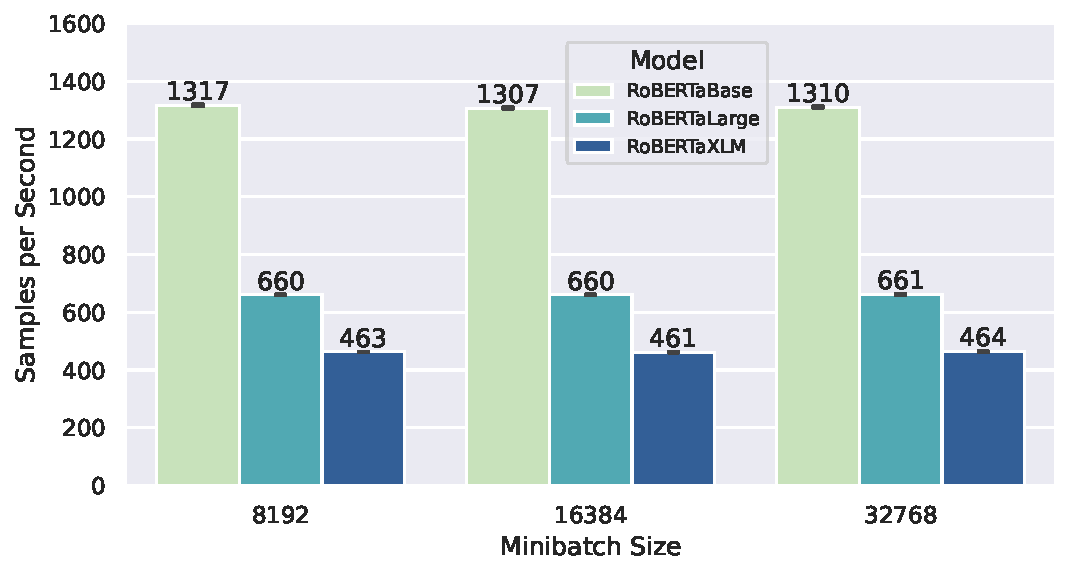
\includegraphics[width=\textwidth]{figures/misc/nlp_1xa10_all-tbs_baseline}
        \vspace{-18pt}
        \caption{NLP 1xA10}
        \label{fig:nlp-1xa10-baseline}
    \end{subfigure}
    \begin{subfigure}[c]{0.23\textwidth}
        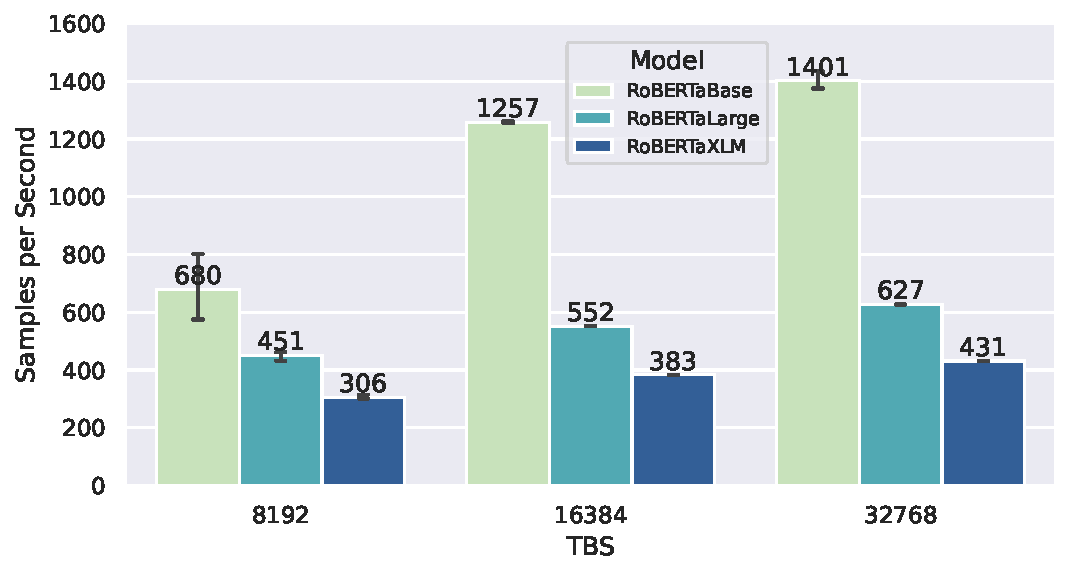
\includegraphics[width=\textwidth]{figures/misc/nlp_2xa10_all-tbs_hivemind}
        \vspace{-18pt}
        \caption{NLP 2xA10} 
        \label{fig:nlp-2xa10-hivemind}
    \end{subfigure}
    \vspace{-10pt}
    \caption{Throughput comparison between single GPU baselines and the Hivemind runs with two GPUs.}
    \label{fig:1x-vs-2xa10-throughput-comparison}
    \vspace*{-6mm}
\end{figure}

Our experimental results in ~\Cref{fig:1x-vs-2xa10-throughput-comparison} show the practical implications of this observation.
For the dual GPU experiments in ~\Cref{fig:cv-2xa10-hivemind,fig:nlp-2xa10-hivemind}, we can see the effect of a TBS increase which improves the total throughput.
Doubling the TBS equals cutting down the per-sample communication cost by two, which leads to the slight increase in performance visible in both CV and NLP experiments.
However, the smallest models, ResNet18 and RoBERTaBase, fluctuate significantly at a TBS of 8K due to a minimum matchmaking time of 5 seconds. 
Whenever all peers accumulate the TBS in less than 5 seconds, the asynchronous thread that tries to match the peers in groups to perform the all-reduce may still need to finish.
This results in an unstable averaging time, which limits the scalability of small models combined with a small TBS.

To illustrate how the TBS and model size affect the individual timings, we visualize the total training time split up into the calculation and communication time in ~\Cref{fig:2xa10-granulartiy}.
CV models are generally computationally more expensive and have a higher granularity than NLP models, which have slightly longer averaging rounds due to the much larger model sizes (cf.~\Cref{tab:experimental-setup-for-model-suitability}).
When comparing the models at the same TBS (e.g., 32K), there is an inconclusive relation between runtime and parameter count.
Some models increase their runtime with parameter count w.r.t. smaller models (RN50 to RN152, RBase to RLrg), while others decrease their runtime (RN152 to WRN101, RLrg to RXLM).
This performance is because not all parameters are the same: A feedforward layer performs one matrix multiplication over the input and its hidden size, while a convolutional layer is more sample-efficient and applies multiple small matrix multiplications over input slices.
Depending on the specific architecture, even models with more parameters can be faster to train due to a more efficient architecture, such as the WideResNet101~\cite{zagoruyko2016wide}.

The communication time between different TBS sizes stays the same, barring the two matchmaking time exceptions (RN18, RBase), as the gradients are accumulated before being sent.
For all other models, doubling the TBS leads to exactly double the amount of work and doubles the granularity. 
With a TBS of 32K, all models have a granularity of at least 4.2 (RXLM) and at most 21.6 (CONV), which show strong scaling potential. 
Therefore, we decided to use a TBS of 32K for all following experiments to ensure that the setup scales before introducing bandwidth and computational limitations.

Summarizing, whether a model is scalable without network bandwidth limitations depends on the minimum time to reach the TBS and on the granularity.
Tuning the TBS is possible to a certain extent but depends on the specific training task and optimizer configuration.

\begin{figure}
    \begin{subfigure}[c]{0.23\textwidth}
        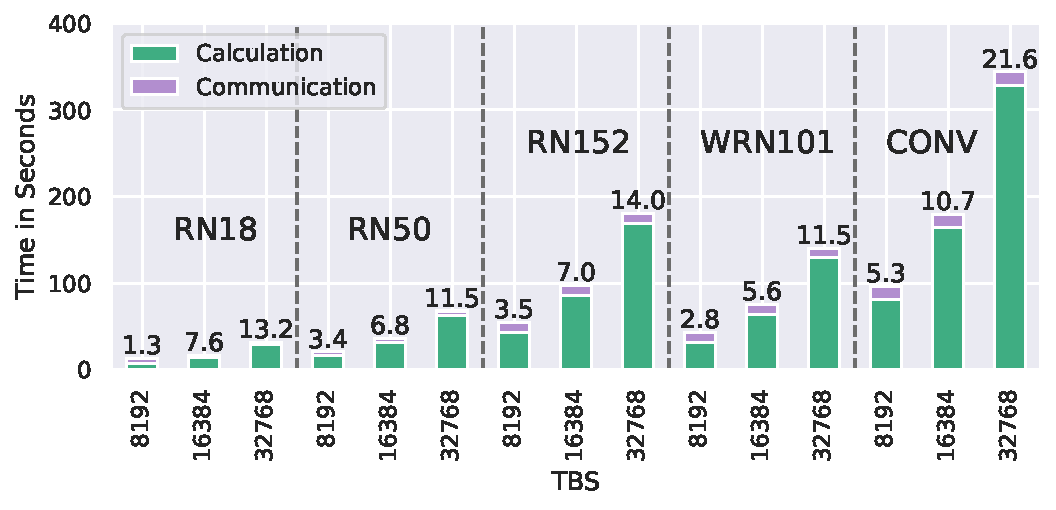
\includegraphics[width=\textwidth]{figures/misc/cv_2xa10_all-tbs_granularity}
        \vspace{-18pt}
        \caption{CV}
        \label{fig:cv-2xa10-granulartiy}
    \end{subfigure}
    \begin{subfigure}[c]{0.23\textwidth}
        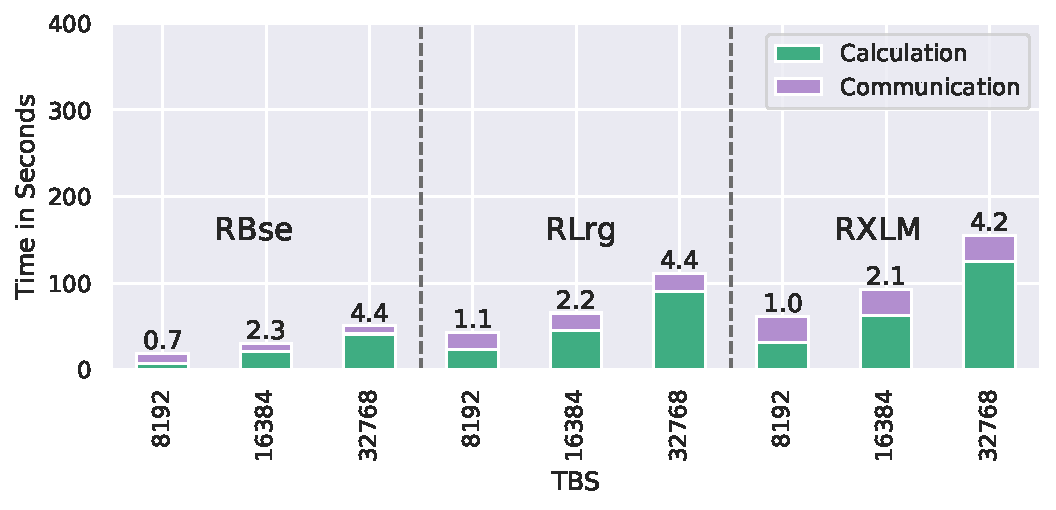
\includegraphics[width=\textwidth]{figures/misc/nlp_2xa10_all-tbs_granularity}
        \vspace{-18pt}
        \caption{NLP} 
        \label{fig:nlp-2xa10-granularity}
    \end{subfigure}
    \vspace{-10pt}
    \caption{TBS vs. total training time on 2xA10s. Granularity is shown above each bar. Dotted lines separate different models.}
    \label{fig:2xa10-granulartiy}
\end{figure}

\begin{figure}
    \begin{subfigure}[c]{0.23\textwidth}
        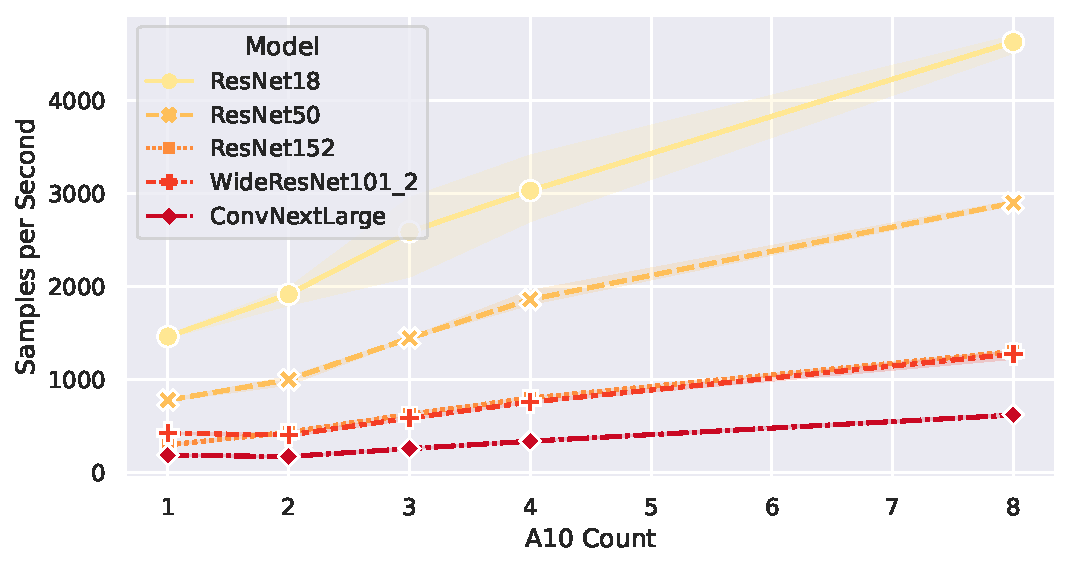
\includegraphics[width=\textwidth]{figures/misc/cv_multi-a10_scalability}
        \vspace{-18pt}
        \caption{CV}
        \label{fig:cv-multi-a10}
    \end{subfigure}
    \begin{subfigure}[c]{0.23\textwidth}
        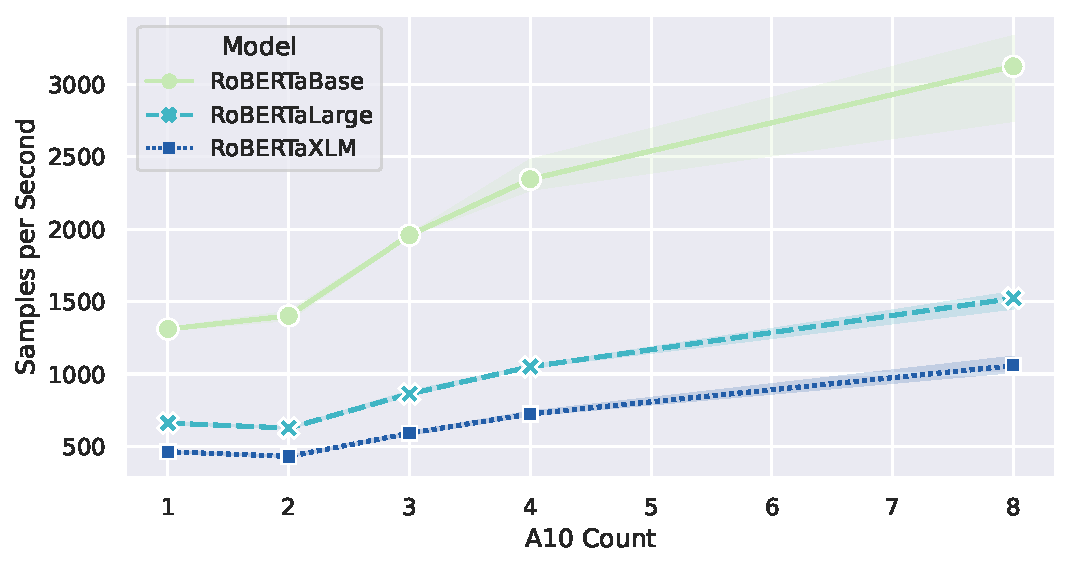
\includegraphics[width=\textwidth]{figures/misc/nlp_multi-a10_scalability}
        \vspace{-18pt}
        \caption{NLP}
        \label{fig:nlp-multi-a10}  
    \end{subfigure}
    \vspace{-10pt}
	\caption{Throughput comparison from 1 to 8 A10 GPUs.}
	\label{fig:multi-a10}
\end{figure}

\begin{table}[]
    \begin{center}
    \scalebox{0.9}{
    \begin{tabular}{l|r|r|r|r}
     & 2 GPUs & 3 GPUs & 4 GPUs & 8 GPUs \\ \hline
    ResNet18         & 1.31x (0.7) & 1.77x (0.6) & 2.07x (0.5) & 3.16x (0.4) \\ 
    ResNet50         & 1.28x (0.6) & 1.86x (0.6) & 2.39x (0.6) & 3.72x (0.5) \\ 
    ResNet152        & 1.46x (0.7) & 2.11x (0.7) & 2.69x (0.7) & 4.37x (0.5) \\ 
    WideResNet101\_2 & 0.95x (0.5) & 1.38x (0.5) & 1.79x (0.4) & 3.01x (0.4) \\ 
    ConvNextLarge    & 0.94x (0.5) & 1.39x (0.5) & 1.82x (0.5) & 3.34x (0.4) \\ \hline
    RoBERTaBase      & 1.07x (0.5) & 1.49x (0.5) & 1.79x (0.4) & 2.38x (0.3) \\ 
    RoBERTaLarge     & 0.95x (0.5) & 1.30x (0.4) & 1.59x (0.4) & 2.30x (0.3) \\
    RoBERTaXLM       & 0.93x (0.5) & 1.28x (0.4) & 1.56x (0.4) & 2.29x (0.3) \\
    \end{tabular} 
    } 
    \end{center} 
    \caption{Baseline speedup for all experiments. Per-GPU contribution in parenthesis.} 
    \label{tab:speedup-multi-a10s}
    \vspace*{-6mm}
\end{table}  
  
\begin{figure}
    \begin{subfigure}[c]{0.23\textwidth}
        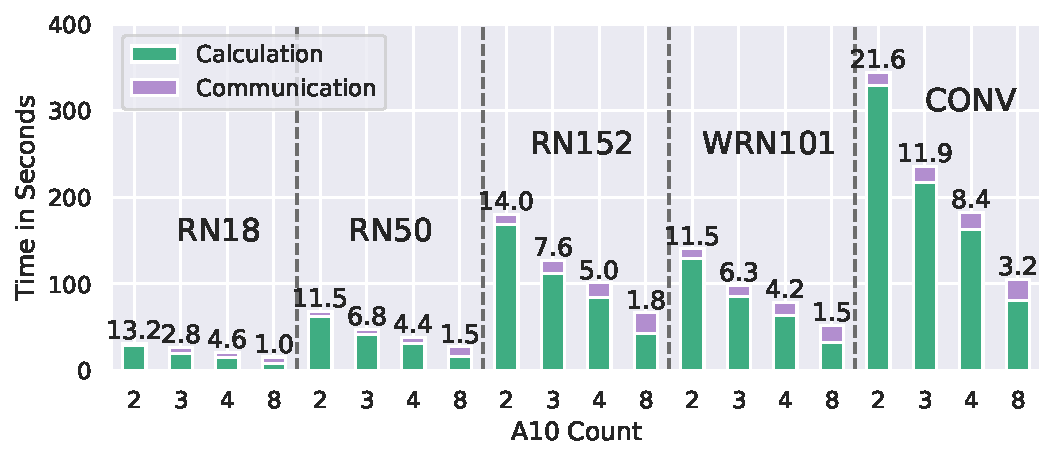
\includegraphics[width=\textwidth]{figures/misc/cv_full-a10_all-tbs_granularity}
        \vspace{-18pt}
        \caption{CV} 
        \label{fig:cv-multi-a10-granularity}
    \end{subfigure}
    \begin{subfigure}[c]{0.23\textwidth}
        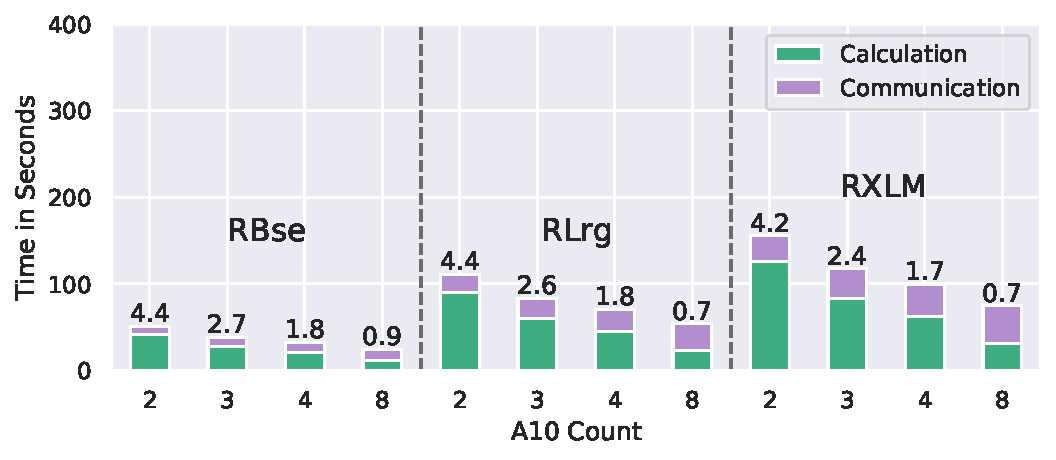
\includegraphics[width=\textwidth]{figures/misc/nlp_full-a10_all-tbs_granularity}
        \vspace{-18pt}
        \caption{NLP}
        \label{fig:nlp-multi-a10-granularity}
    \end{subfigure} 
    \vspace{-10pt} 
    \caption{Multi-GPU scalability at 32K TBS. Granularity is shown above each bar.Dotted lines separate different models.}
    \label{fig:multi-a10-granulartiy}
    \vspace*{-4mm}
\end{figure}  

\textbf{(3) Per-GPU speedup decreases with low granularity.}
To evaluate the scalability with additional hardware, we profile all models on 2,3,4, and 8 GPUs with a TBS of 32K.
~\Cref{fig:multi-a10} shows the throughput for all models in the different hardware scenarios with the respective speedup in ~\Cref{tab:speedup-multi-a10s}.
Generally, all models scale well regardless of size, with the best speedup of 4.37x (ResNet152) and the lowest at 2.29x (RoBERTaXLM) with 8 GPUs.
There is a visible trend in the per-GPU contribution to the speedup ($\frac{\text{speedup}}{\#\text{GPUs}}$).
The more GPUs we add, the lower the contribution, e.g., ResNet18 goes from 0.7 to 0.4 with two to eight GPUs, respectively.
This decrease is likely to continue due to a granularity of 1.0 at 8 GPUs (\Cref{fig:cv-multi-a10-granularity}), as doubling the GPUs would, at best, increase the throughput by 33\% by halving the calculation time.
However, the more computationally expensive the models are, the slower the per-GPU contribution falls off and the larger the granularity is (ResNet152, ConvNextLarge).
This does not hold true for our NLP models (\Cref{fig:nlp-multi-a10-granularity}); while they have increasingly more model parameters, the only difference between the two biggest models, RoBERTaLarge and RoBERTaXLM, is the vocabulary size increase of 50K to 250K.
Due to the attention mechanism of the transformer architecture, the forward pass is not affected by the increased embedding size, but the backward pass is.
This results in a smaller increase of the calculation time while communication increases linearly with the number of parameters.

Additionally, we see the slight drop in throughput when comparing the single GPU and dual GPU experiments for most larger models (\Cref{fig:multi-a10}), which stems from observation \textbf{(1)} of the initial Hivemind penalty.  

We also observe that with each subsequent doubling of GPUs, the calculation time is halved, while the communication increases sub-linearly due to the more efficient group-based all-reduce of MoshpitSGD~\cite{ryabinin2021moshpit}.
For example, the averaging step for the RoBERTaXLM on 2xA10 takes 5 seconds per GPU (10s total), while the 8xA10 averaging step takes 1.8 seconds per GPU (14.4s total).

In summary, all models show a speedup but have a decreasing per-GPU contribution due to smaller granularity with more GPUs.
Therefore, the larger the model and TBS, the greater the scaling potential.
High granularity is a good indicator of scalability, and since the communication time only increases linearly with additional peers (cf.~\Cref{ssec:hivemind}), knowing the initial calculation time is a good indicator of future throughput.
Under the optimal conditions of good compute performance and an interconnect with relatively high bandwidth, scaling was not a problem.
But what happens under less favorable conditions in geo-distributed settings?